\documentclass{article}
\usepackage[UTF8]{ctex}
% Replace `letterpaper' with`a4paper' for UK/EU standard size
\usepackage[a4paper,top=2cm,bottom=2cm,left=3cm,right=3cm,marginparwidth=1.75cm]{geometry}

% Useful packages
\usepackage{amsmath}
\usepackage{graphicx}
\usepackage[colorlinks=true, allcolors=blue]{hyperref}
\usepackage{graphicx} %插入图片的宏包
\usepackage{float} %设置图片浮动位置的宏包
\usepackage{subfigure} %插入多图时用子图显示的宏包
\usepackage{parskip}
\usepackage{indentfirst} 
\setlength{\parindent}{2em}
\usepackage{hyperref}  
\usepackage{tikz}
\allowdisplaybreaks
\usepackage{multirow}
\usepackage{amsmath}
\usepackage{amsfonts,amssymb} 
\usepackage{xcolor} % 用于显示颜色
\usepackage{listings} % 用于插入代码
\lstset{
	basicstyle          =   \sffamily,          % 基本代码风格
	keywordstyle        =   \bfseries,          % 关键字风格
	commentstyle        =   \rmfamily\itshape,  % 注释的风格,斜体
	stringstyle         =   \ttfamily,  % 字符串风格
	flexiblecolumns,                % 别问为什么,加上这个
	numbers             =   left,   % 行号的位置在左边
	showspaces          =   false,  % 是否显示空格,显示了有点乱,所以不现实了
	numberstyle         =   \zihao{-5}\ttfamily,    % 行号的样式,小五号,tt等宽字体
	showstringspaces    =   false,
	captionpos          =   t,      % 这段代码的名字所呈现的位置,t指的是top上面
	frame               =   lrtb,   % 显示边框
}

\lstdefinestyle{Python}{
	language        =   Python, % 语言选Python
	basicstyle      =   \zihao{-5}\ttfamily,
	numberstyle     =   \zihao{-5}\ttfamily,
	keywordstyle    =   \color{blue},
	keywordstyle    =   [2] \color{teal},
	stringstyle     =   \color{magenta},
	commentstyle    =   \color{red}\ttfamily,
	breaklines      =   true,   % 自动换行,建议不要写太长的行
	columns         =   fixed,  % 如果不加这一句,字间距就不固定,很丑,必须加
	basewidth       =   0.5em,
}

\title{Project-1 Pacman实验报告}
\author{林子开 21307110161}
\begin{document}
	\maketitle
	\tableofcontents

\section{Restate the Basic Global Thresholding using the histogram}
Given the histogram of an image, we assume $P(i)$ as the proportion 
of pixel(s) with intensity $i$ in the image. We can implement the BGT algorithm 
more efficiently based on this histogram.

The algorithm is as follows:
\begin{enumerate}
    \item Select the initial threshold $T_0$ as the mean intensity
        $$T =\mu = \sum_{i=0}^{255} i P(i)$$
    \item Calculate respectively the mean intensity values for Foreground and Background,
        which are $$\mu_{FG}=\frac{\sum_{i=0}^{T_k-1}iP(i)}{\sum_{i=0}^{T_k-1}P(i)}
        ,\, \mu_{BK}=\frac{\sum_{i=T_k}^{255}iP(i)}{\sum_{i=T_k}^{255}P(i)}$$
    \item Set a new threshold $$T_{k+1} = \frac{\mu_{FG}+\mu_{Bk}}{2}$$
    \item Repeat steps 2-3, until $|T_{k+1}-T_k|<\varepsilon$, 
        where $\varepsilon$ is a given small number.
\end{enumerate}


%=================================================================================

\section{Locally adaptive thresholding} 
\subsection{算法实现简介}
在本题中,我首先调用了在第一次作业中实现的local-list函数,该函数能够
根据所输入的patchSize,返回对应于图像中所有像素点的局部灰度值直方图。
此外,我也提前生成了对应于patchSize=$25,50,100,150$的局部直方图文件,
也可以直接导入,节省时间。

对于每个像素点以及该像素点所对应的局部直方图,我使用了\textbf{OTSU算法},
找出该局部直方图的最优阈值$T$,再根据$T$与该像素点灰度值的大小关系,返回0或255。

具体的Python代码如下一小节所示。

\subsection{Python代码}
\lstinputlisting[style = Python,
caption={Python codes for locally adaptive thresholding based on OTSU},
label = {OTSU}]{codes/exercise_2.py} 

\subsection{测试案例:肝脏核磁共振影像}
下面,我们使用如下的肝脏核磁共振影像作为测试案例:
\begin{figure}[H]
	\centering
	{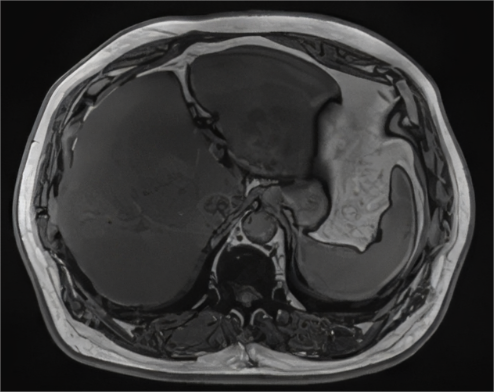
\includegraphics[width=0.49\textwidth]{codes//肝脏.png}} 
	\caption{肝脏核磁共振影像}
\end{figure}
注意到,该影像的对比度不是特别高。此外,该肝脏(目测)有一些密度发生改变的地方,
有可能代表着某些器质性病变,需要将这些可能病变的部位更加明显地展示出来。

我们使用局部自适应二值化的算法,分别取局部直方图的patchSize=$25,50,100,150$的情况
进行测试,测试结果如下:

\begin{figure}[H]
    \centering
    \subfigure[patchSize = 25]
	{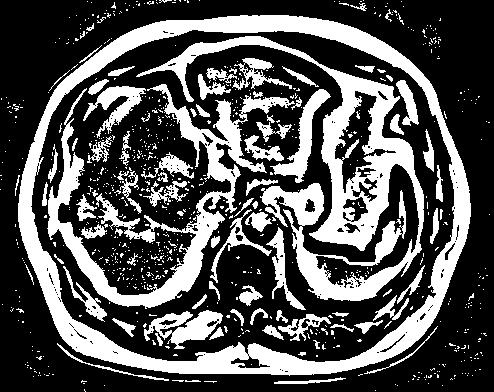
\includegraphics[width=0.49\textwidth]{codes//exercise2_肝脏.png_patchSize=25.jpg}}
    \,    
    \subfigure[patchSize = 50]
    {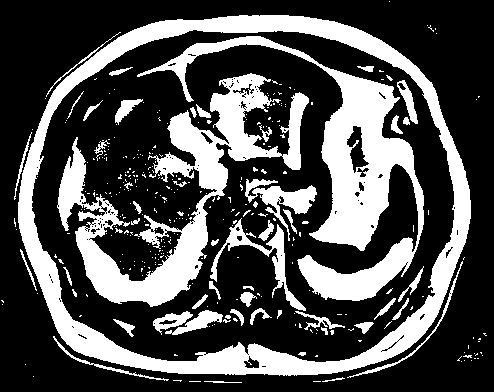
\includegraphics[width=0.49\textwidth]{codes//exercise2_肝脏.png_patchSize=50.jpg}}
    \,
    \subfigure[patchSize = 100]
    {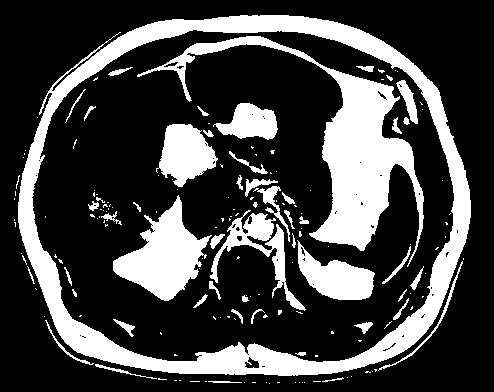
\includegraphics[width=0.49\textwidth]{codes//exercise2_肝脏.png_patchSize=100.jpg}}
    \,    
    \subfigure[patchSize = 150]
    {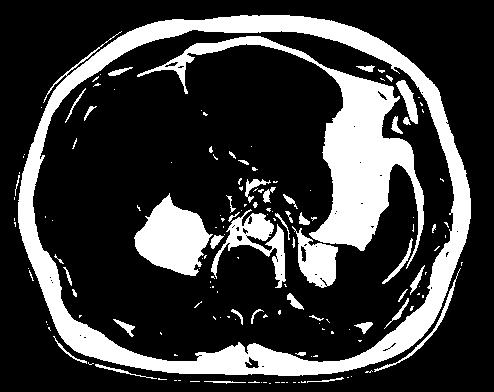
\includegraphics[width=0.49\textwidth]{codes//exercise2_肝脏.png_patchSize=150.jpg}}
    \caption{locally adaptive thresholding with different patch size}
\end{figure}

观察以上四个图像可以发现,patchSize选取为25时,图像非常混乱,展示了过多无效的细节;
patchSize选取为100和150时,则又出现大面积的黑色与白色,提供的关于可能病变区域的信息不足。
相较而言,patchSize选取为50时的图像中,肝脏的整体轮廓仍然是清晰的,且展示了
肝脏各个区域在局部的密度变化的情况,更有助于发现可能病变的位置。因此,在本次实验所选取的4个
patchSize中,我推荐使用patchSize=50。


%==================================================================================

\section{线性插值算法:放大图片分辨率}

\subsection{算法实现简介}
我们定义:将图片的分辨率放大$N$倍,就是向原本相邻的两个像素点之间插入$N-1$个像素点,
也即将总的像素点数量扩大到原来的$N^2$倍。

我实现线性插值的方法是:先在第一个(横向的)维度上进行线性插值,
再在第二个(纵向的)维度上进行线性插值,最终完成对整张图片的分辨率扩大。
以$N=3$为例,示意图如下:

\begin{figure}[H]
	\centering
	{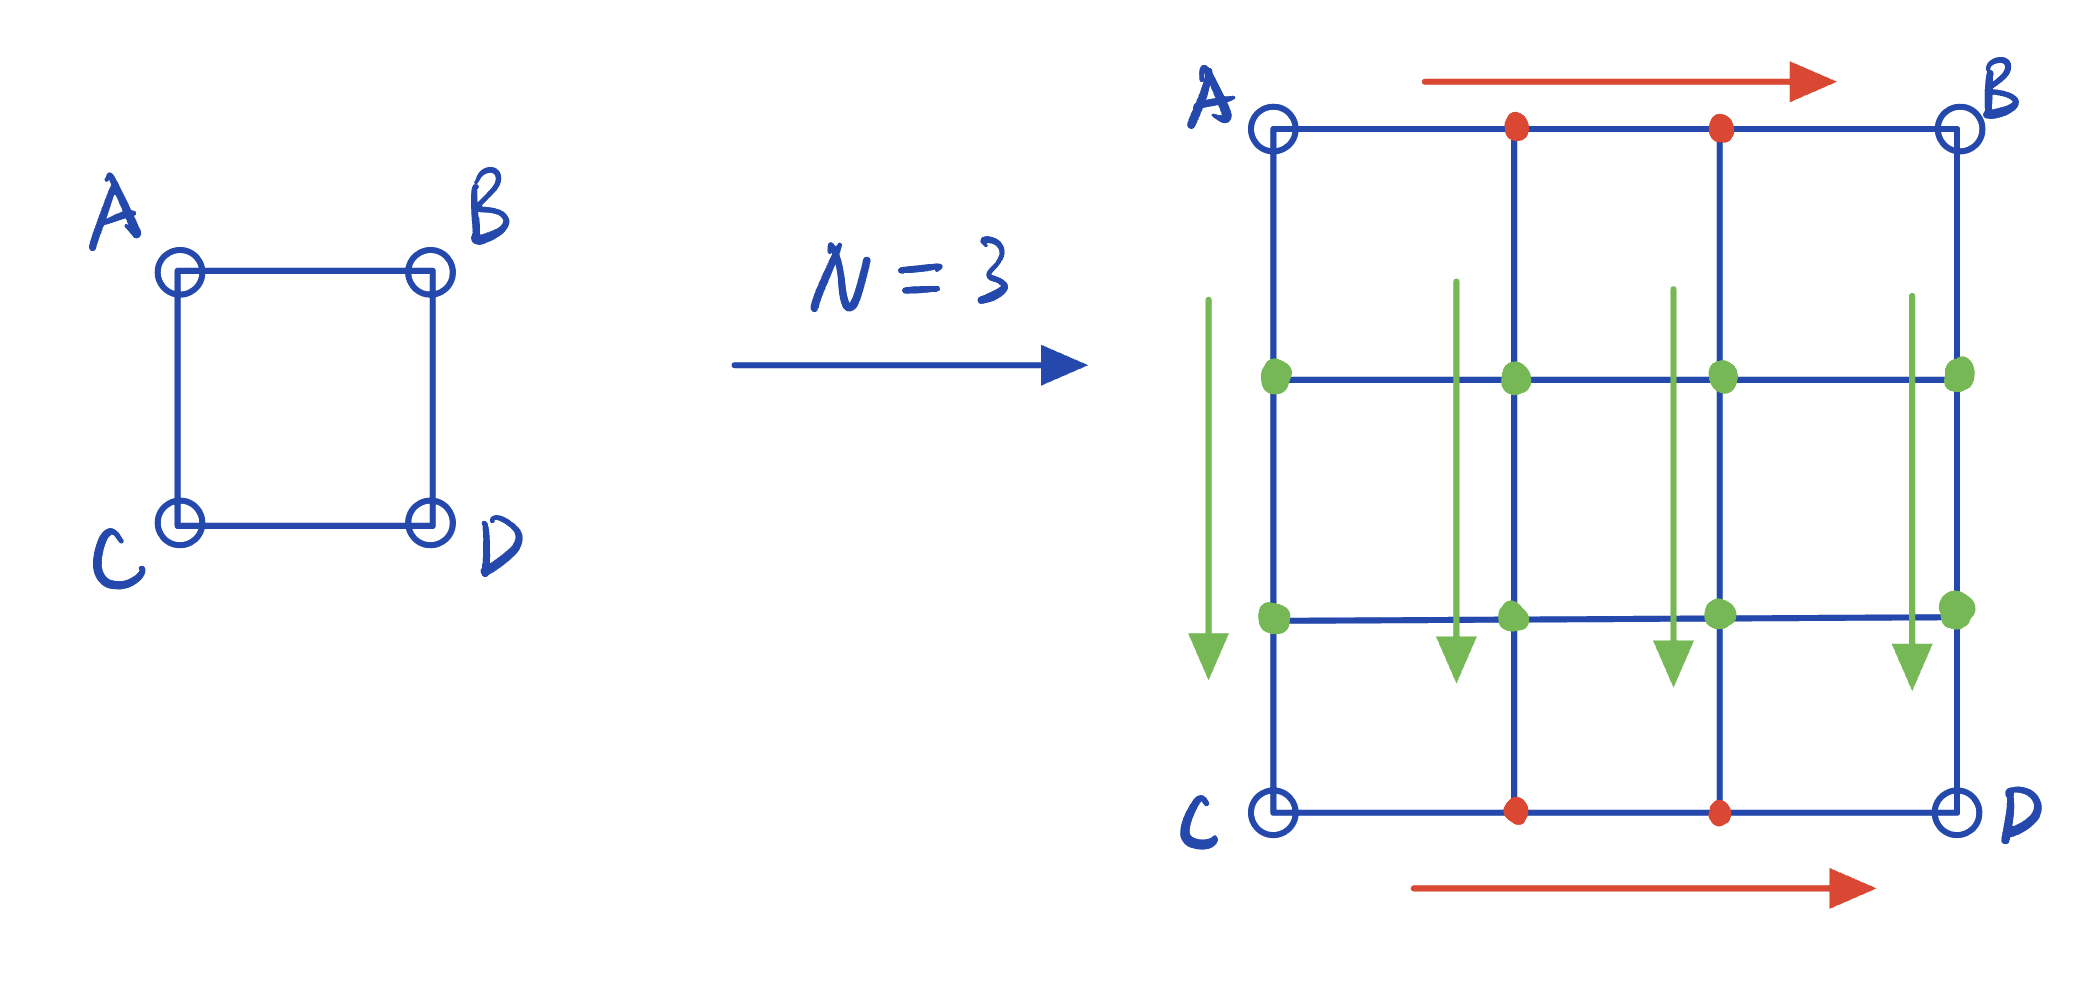
\includegraphics[width=0.75\textwidth]{算法示意图.jpg}} 
	\caption{线性插值算法示意图}
\end{figure}

假设$A, B, C, D$是原图片中相邻的4个像素点,在新图片中,原本相邻的像素点之间
被插入了$N-1=2$个新像素点。
我们首先沿着第一个方向(横向),对$AB$边上的点以及$CD$边上的点(图中红点)进行线性插值,
$AB$边上的点的灰度值是$A$点和$B$点的灰度值的线性组合,$CD$边同理。

然后,沿着第二个方向(纵向),对内部的其他的点(绿点)进行线性插值,这些内部点的
灰度值都是其上方的红点(或者原图像素点)及其下方的红点(或者原图像素点)的灰度值的线性组合。

实现线性插值算法的Python代码如下一小节所示。

\subsection{Python代码}

\lstinputlisting[style = Python,
caption={Python codes for linear interpolation},
label = {Linear}]{codes/exercise_3.py} 

\subsection{测试案例:86版西游记剧照}
该剧照的原始分辨率为$329\times 259$,通过上面的算法,将其分辨率分别扩大
到$N=2,3,4$,原图以及分别率扩大后的效果如下所示:

\begin{figure}[]
    \centering
    \subfigure[原图]
	{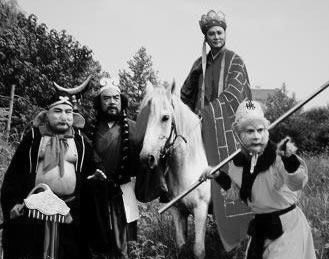
\includegraphics[width=0.2\textwidth]{codes//86版西游记模糊剧照.png}}
    \,    
    \subfigure[放大倍数N = 2]
    {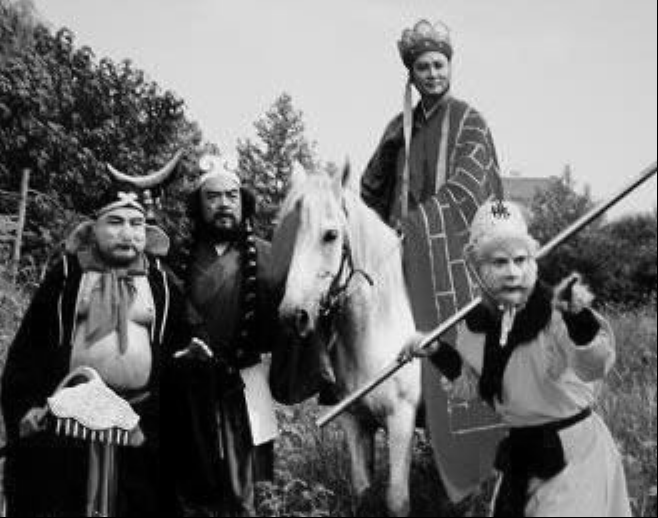
\includegraphics[width=0.4\textwidth]{codes//exercise_3_线性插值_86版西游记模糊剧照.png_N=2.png}}
    \,
    \subfigure[放大倍数N = 3]
    {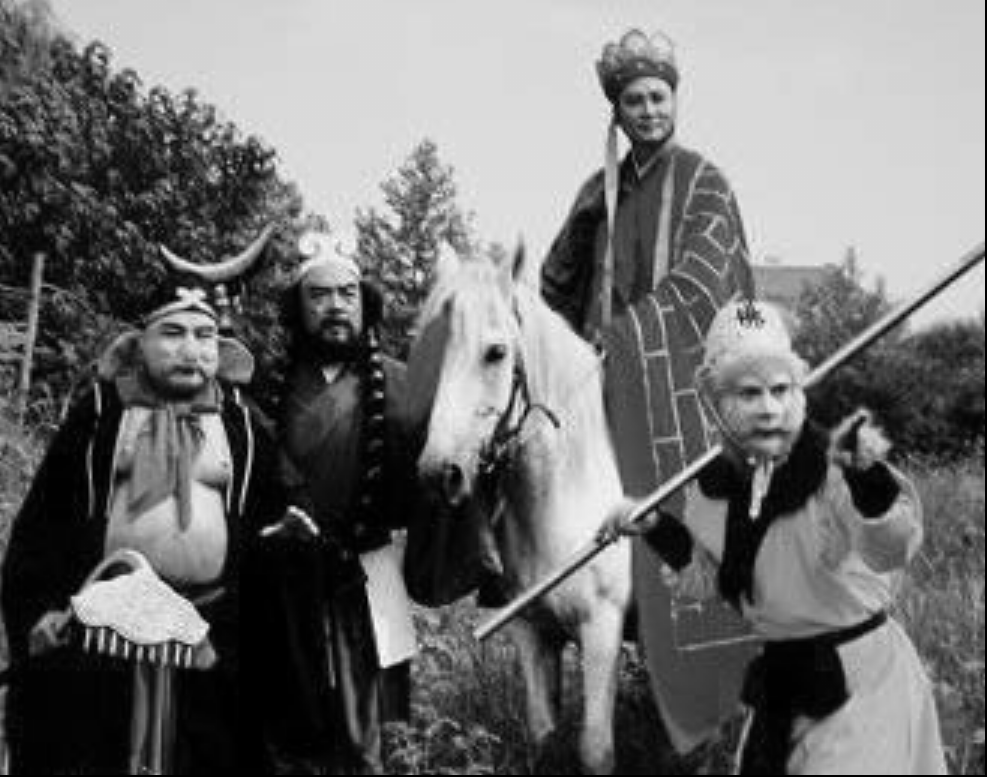
\includegraphics[width=0.6\textwidth]{codes//exercise_3_线性插值_86版西游记模糊剧照.png_N=3.png}}
    \,    
    \subfigure[放大倍数N = 4]
    {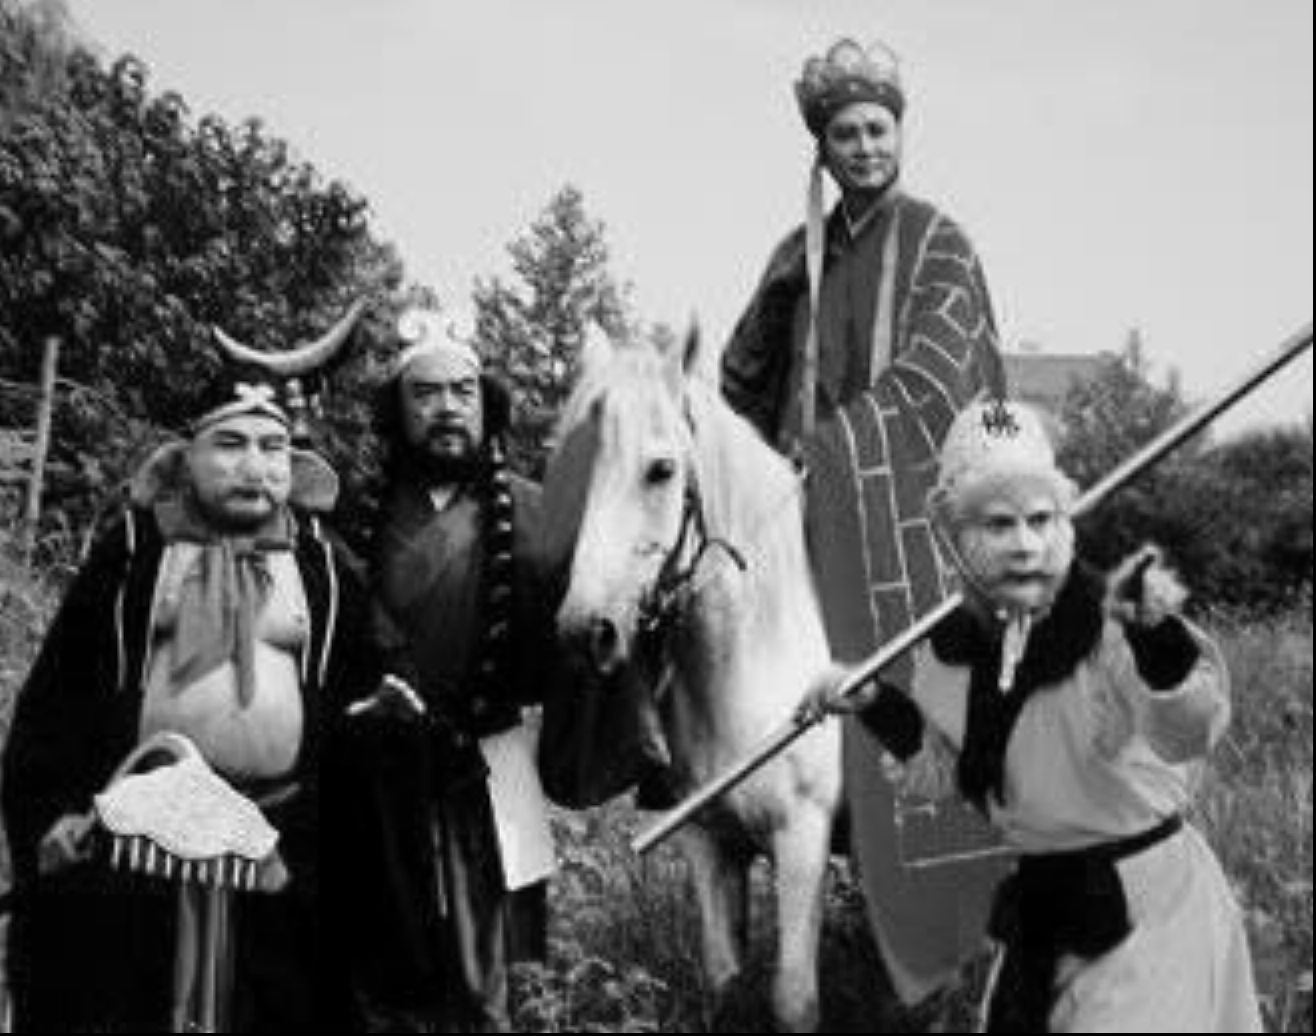
\includegraphics[width=0.8\textwidth]{codes//exercise_3_线性插值_86版西游记模糊剧照.png_N=4.png}}
    \caption{locally adaptive thresholding with different patch size}
\end{figure}


可以看出,经过线性插值之后,分辨率放大后的图片仍然保持较好的清晰度,
将这些图片放大后没有出现“棋盘状”的纹路,说明线性插值后图片的分辨率仍然较好。




\end{document}

% \begin{figure}[H]
% 	\centering
% 	{\includegraphics[width=0.35\textwidth]{image//ignorance.png}} 
% 	\caption{}
% \end{figure}


% \lstinputlisting[style = Python,
% caption={Python codes},
% label = {efficient},
% linerange={110-125}]{exercise3.py} 


% \begin{figure}[H]
%     \centering
%     \subfigure[patch size = 11]
%     {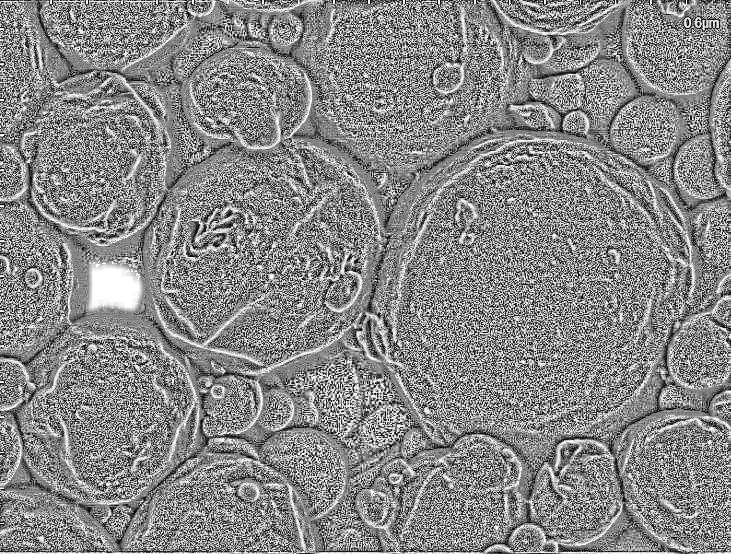
\includegraphics[width=0.49\textwidth]{image//local equalization with patch size = 11.jpg}}
%     \,    
%     \subfigure[patch size = 51]
%     {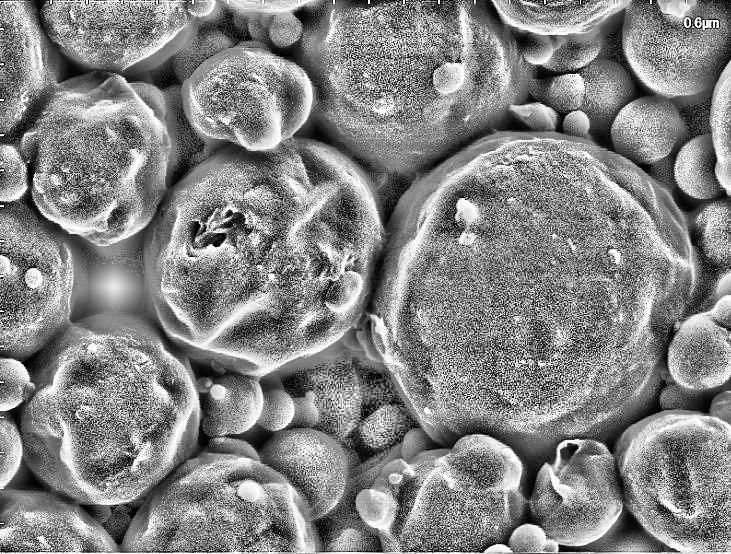
\includegraphics[width=0.49\textwidth]{image//local equalization with patch size = 51.jpg}}
%     \,
%     \subfigure[patch size = 151]
%     {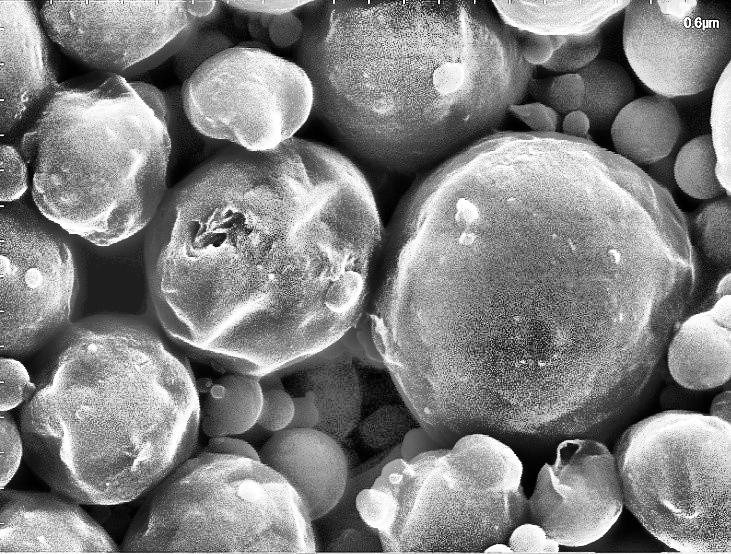
\includegraphics[width=0.49\textwidth]{image//local equalization with patch size = 151.jpg}}
%     \,    
%     \subfigure[patch size = 201]
%     {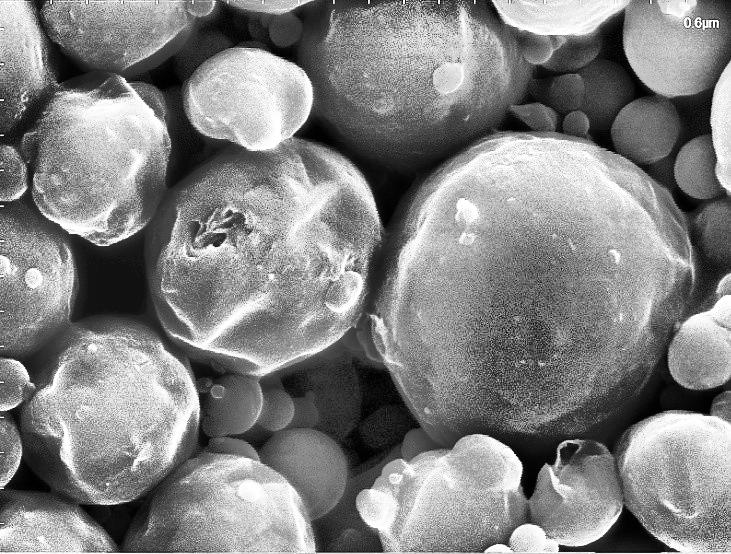
\includegraphics[width=0.49\textwidth]{image//local equalization with patch size = 201.jpg}}
%     \caption{local equalization with different patch sizes}
% \end{figure}
